{\color{indiagreen}\subsection{Opisovanje nihanja}}
Nihanje je periodično gibanje.\\
\textbf{Matematično nihalo}(nitno/težno)\\
%\begin{center}
%	\includegraphics[width=15cm, height=15cm,keepaspectratio=true]{Nihanje.png}
%\end{center}
1 perioda je 1 nihaj, ki je od ene skrajne lege do druge skrajne lege in nazaj.\\
\begin{align*}
	R &\dots \text{ravnovesna lega}\\
	A &\dots \text{amplitudna lega}\\
	t_0 &\dots \text{nihanj čas}\\
	\nu &= \frac{N}{t} = \frac{\text{število nihajev}}{\text{čas}}\\
	{\color{bostonuniversityred}\nu} &= {\color{bostonuniversityred}\frac{1}{t_0}}\\
	s &\dots \text{odmik[cm]}\\
	s_0 &\dots \text{amplituda[cm]}\\
\end{align*}
\textbf{Vzmetno nihalo}\\
%\begin{center}
%	\includegraphics[width=15cm, height=15cm,keepaspectratio=true]{Nihanje2.png}
%\end{center}
Telo kroži enakomerno.\\
%\begin{center}
%	\includegraphics[width=15cm, height=15cm,keepaspectratio=true]{Nihanje3.png}
%\end{center}
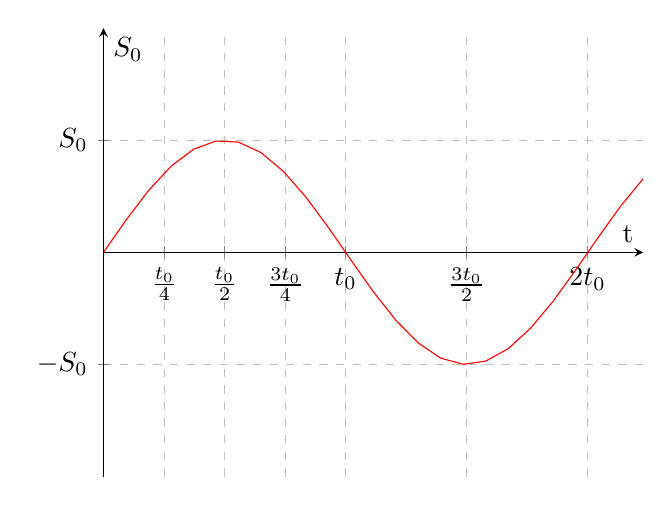
\begin{tikzpicture}
	\begin{axis}[
	    xlabel={t},
	    ylabel={$S_0$},
	    xmin=0, xmax=7,
	    ymin=-2, ymax=2,
	    xtick={0,0.79, 1.57, 2.36, 3.14, 4.71, 6.28},
	    ytick={-1,0,1},
	    xticklabels={0,$\frac{t_0}{4}$, $\frac{t_0}{2}$, $\frac{3t_0}{4}$, $t_0$, $\frac{3t_0}{2}$, $2t_0$},
	    yticklabels={$-S_0$, 0, $S_0$},
	    ymajorgrids=true,
	    xmajorgrids=true,
	    grid style=dashed,
	    axis lines=middle,
	]
	\addplot[domain=0:7,red] {sin(deg(x))};
	\end{axis}
\end{tikzpicture}\\
%\begin{center}
%	\includegraphics[width=15cm, height=15cm,keepaspectratio=true]{Nihanje4.png}
%\end{center}
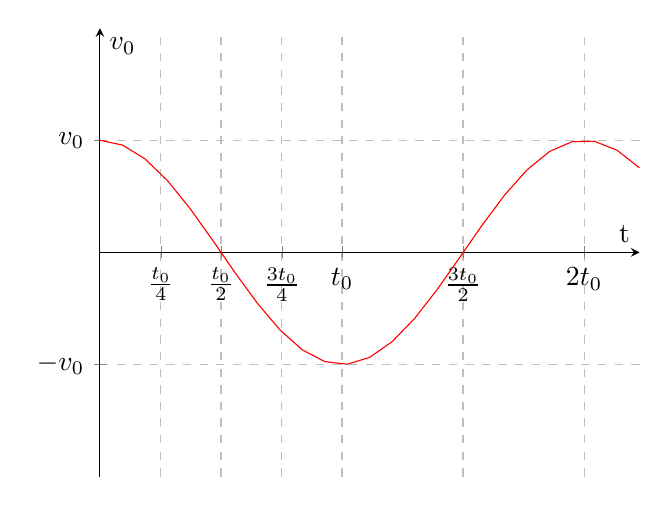
\begin{tikzpicture}
	\begin{axis}[
	    xlabel={t},
	    ylabel={$v_0$},
	    xmin=0, xmax=7,
	    ymin=-2, ymax=2,
	    xtick={0,0.79, 1.57, 2.36, 3.14, 4.71, 6.28},
	    ytick={-1,0,1},
	    xticklabels={0,$\frac{t_0}{4}$, $\frac{t_0}{2}$, $\frac{3t_0}{4}$, $t_0$, $\frac{3t_0}{2}$, $2t_0$},
	    yticklabels={$-v_0$, 0, $v_0$},
	    ymajorgrids=true,
	    xmajorgrids=true,
	    grid style=dashed,
	    axis lines=middle,
	]
	\addplot[domain=0:7,red] {cos(deg(x))};
	\end{axis}
\end{tikzpicture}\\
%\begin{center}
%	\includegraphics[width=15cm, height=15cm,keepaspectratio=true]{Nihanje3.png}
%\end{center}
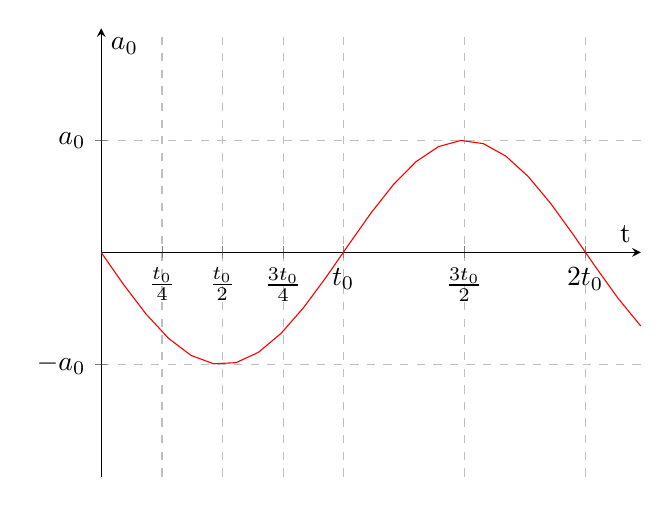
\begin{tikzpicture}
	\begin{axis}[
	    xlabel={t},
	    ylabel={$a_0$},
	    xmin=0, xmax=7,
	    ymin=-2, ymax=2,
	    xtick={0,0.79, 1.57, 2.36, 3.14, 4.71, 6.28},
	    ytick={-1,0,1},
	    xticklabels={0,$\frac{t_0}{4}$, $\frac{t_0}{2}$, $\frac{3t_0}{4}$, $t_0$, $\frac{3t_0}{2}$, $2t_0$},
	    yticklabels={$-a_0$, 0, $a_0$},
	    ymajorgrids=true,
	    xmajorgrids=true,
	    grid style=dashed,
	    axis lines=middle,
	]
	\addplot[domain=0:7,red] {-sin(deg(x))};
	\end{axis}
\end{tikzpicture}\\
\begin{align*}
	{\color{bostonuniversityred}S} &= {\color{bostonuniversityred}S_0 \sin(\omega t)}\\
	\rho = \omega t \dots &\text{{\color{bostonuniversityred}POMNI:} To ni isti kot, kot pri nihanju, to je kot pri kroženju.}\\
	{\color{bostonuniversityred}v} &= {\color{bostonuniversityred}v_0 \cos(\omega t)}\\
	{\color{bostonuniversityred}v_0} &= {\color{bostonuniversityred}\omega S_0} \dots \text{Odvajamo po času.}\\
	a &= -a_0 \sin(\omega t)\\
	{\color{bostonuniversityred}a} = {\color{bostonuniversityred}\omega v_0} &= {\color{bostonuniversityred}\omega^2 s_0} = {\color{bostonuniversityred}\frac{v_0^2}{s_0}}\\ 
	\omega &= 2 \pi \nu\\
\end{align*}
